\documentclass[a4paper,11pt]{article}
\usepackage[margin=20mm]{geometry}
\usepackage{amsmath,amssymb,graphicx,booktabs,array,float,hyperref}
\hypersetup{hidelinks}
\setlength{\parindent}{0pt}
\setlength{\parskip}{5pt}
\renewcommand{\arraystretch}{1.14}
\setlength{\tabcolsep}{4pt}
\begin{document}
\thispagestyle{empty}
\begin{center}{\Large\bfseries Beihang University\\School of Mathematical Sciences\\Laboratory Report}\end{center}
{\small Detailed derivations, results and analysis continue on the following pages.}\par
\vspace{3mm}
\begin{tabular}{|p{.22\linewidth}|p{.22\linewidth}|p{.22\linewidth}|p{.22\linewidth}|}\hline
\multicolumn{2}{|p{.47\linewidth}|}{Course: Numerical Analysis Computer Laboratory} & \multicolumn{2}{p{.43\linewidth}|}{Least Squares and Best Square Approximation}\\\hline
\multicolumn{4}{|l|}{Experiment type: Demonstration [ ] Verification [ ] Comprehensive [ ] Design [ ]}\\\hline
Class: 230116 & \multicolumn{2}{l|}{Name: yule yang} & Student ID: 23376268\\\hline
Lab date: 2026.10.17 & \multicolumn{2}{l|}{Instructor:} & Grade:\\\hline

\multicolumn{4}{|p{.95\linewidth}|}{\textbf{Experimental environment}\par macOS on Apple Silicon; Python with NumPy and SciPy; Matplotlib for plots. AI assistance: Codex. Exact package versions and measured results are archived with the experiment.\par\vspace{4mm}}\\\hline
\multicolumn{4}{|p{.95\linewidth}|}{\textbf{Objectives and content}\par Complete all seven experiments: the overdetermined system, line fitting, two population models, three continuous projections, and separate upper and lower RAE2822 airfoil fits.\par\vspace{4mm}}\\\hline
\multicolumn{4}{|p{.95\linewidth}|}{\textbf{Procedure and results}\par All seven experiments were executed and independently checked. The literal system gives RSS 4.1808988764. The fitted line has RSS 94.186046512. The quadratic log population model substantially reduces the log residual. All 129 supplied airfoil coordinates are retained.\par\vspace{4mm}}\\\hline
\multicolumn{4}{|p{.95\linewidth}|}{\textbf{Analysis and conclusions}\par Projection orthogonality explains discrete and continuous least squares. Stable QR is preferable to forming normal equations for poorly scaled designs. Population fitting is performed in log space; airfoil surfaces are split by contour order, not the sign of the ordinate.\par\vspace{4mm}}\\\hline
\end{tabular}
\clearpage
\section*{1 Scope and least squares methods}
This report completes Experiments 1.1, 1.2, 1.3, 2.1, 2.2, 2.3 and 3.1 in the supplied seven page handout. All numerical inputs come from that PDF: five line points, 24 population observations from 1790 to 2020, and 129 airfoil coordinates. No external dataset is substituted.

\[\min_c\|Ac-b\|_2^2,\qquad A^T(Ac-b)=0,\qquad A^TAc=A^Tb.\]
Differentiating the quadratic objective gives the normal equations. When the columns are independent the Gram matrix is positive definite, giving a unique least squares solution. The residual need not vanish, but is orthogonal to every design column.

\[A=QR,\quad Q^TQ=I,\qquad Rc=Q^Tb.\]
An explicit Householder QR implementation is compared with NumPy least squares and with normal equations solved by Gaussian elimination with partial pivoting. No inverse is formed. The hand coded QR is the principal computational solution; the normal equations are included to satisfy the mathematical derivation and to examine conditioning.

\[\kappa_2(A^TA)=\kappa_2(A)^2\quad\text{for full column rank }A.\]
A subtle source issue occurs in Experiment 1.1: the third equation prints x1 + x2 + 2x2 = 2. Its literal row is (1,3,0). A plausible correction is x1 + x2 + 2x3 = 2, giving row (1,1,2). The literal reading is the main answer; the alternative is separately solved and labeled rather than silently replacing the supplied equation.

For continuous problems the residual is orthogonal in an integral inner product. Continuous projections minimize integrated squared error over the full interval; they are not interpolation at selected nodes. Numerical quadrature is used only to verify the derived exact answers.

\clearpage
\section*{2 Experiment 1 1 overdetermined system}
\subsection*{Literal printed equation}
\[A=\begin{pmatrix}1&2&4\\2&1&1\\1&3&0\\1&-1&-2\end{pmatrix},\qquad b=\begin{pmatrix}-1\\4\\2\\1\end{pmatrix}.\]
\[A^TA=\begin{pmatrix}7&6&4\\6&15&11\\4&11&21\end{pmatrix},\qquad A^Tb=\begin{pmatrix}10\\7\\-2\end{pmatrix}.\]
\[\widehat{x}=\begin{pmatrix}1.5213483\\0.22808989\\-0.50449438\end{pmatrix},\qquad r=b-A\widehat{x}=\begin{pmatrix}-0.95955056\\1.2337079\\-0.20561798\\-1.3022472\end{pmatrix}.\]
Residual sum of squares = 4.180898876404. Full precision coefficients and residuals are saved in results.json.

\subsection*{Possible corrected equation}
\[A=\begin{pmatrix}1&2&4\\2&1&1\\1&1&2\\1&-1&-2\end{pmatrix},\qquad b=\begin{pmatrix}-1\\4\\2\\1\end{pmatrix}.\]
\[A^TA=\begin{pmatrix}7&4&6\\4&7&13\\6&13&25\end{pmatrix},\qquad A^Tb=\begin{pmatrix}10\\3\\2\end{pmatrix}.\]
\[\widehat{x}=\begin{pmatrix}1\\4.5\\-2.5\end{pmatrix},\qquad r=b-A\widehat{x}=\begin{pmatrix}-1\\0\\1.5\\-0.5\end{pmatrix}.\]
Residual sum of squares = 3.500000000000. Full precision coefficients and residuals are saved in results.json.

For the literal system the exact coefficient vector is (1354/890, 203/890, -449/890), and RSS = 3721/890. For the alternative it is (1, 9/2, -5/2), and RSS = 7/2. Both residuals satisfy the appropriate normal orthogonality condition; their RSS values cannot be compared as competing fits to the same design because the two designs differ.

\clearpage
\section*{3 Experiment 1 2 fitted line}
Using columns 1 and x, the data are fitted by a + b x with equal weights on all five observations. The normal system and exact rational solution are:

\[\begin{pmatrix}5&151\\151&4629\end{pmatrix}\begin{pmatrix}a\\b\end{pmatrix}=\begin{pmatrix}720\\22240\end{pmatrix}.\]
\[a=-\frac{3170}{43},\qquad b=\frac{310}{43},\qquad \widehat{y}(x)=-73.72093023+7.209302326x.\]
{\small\begin{tabular}{p{0.232\linewidth}p{0.232\linewidth}p{0.232\linewidth}p{0.232\linewidth}}\toprule
x & Observed y & Fitted y & Residual\\\midrule
25 & 110 & 106.511628 & 3.488372\\
27 & 115 & 120.930233 & -5.930233\\
31 & 155 & 149.767442 & 5.232558\\
33 & 160 & 164.186047 & -4.186047\\
35 & 180 & 178.604651 & 1.395349\\
\bottomrule\end{tabular}}\par
\[\operatorname{RSS}=\frac{4050}{43}=94.18604651.\]
\begin{figure}[H]\centering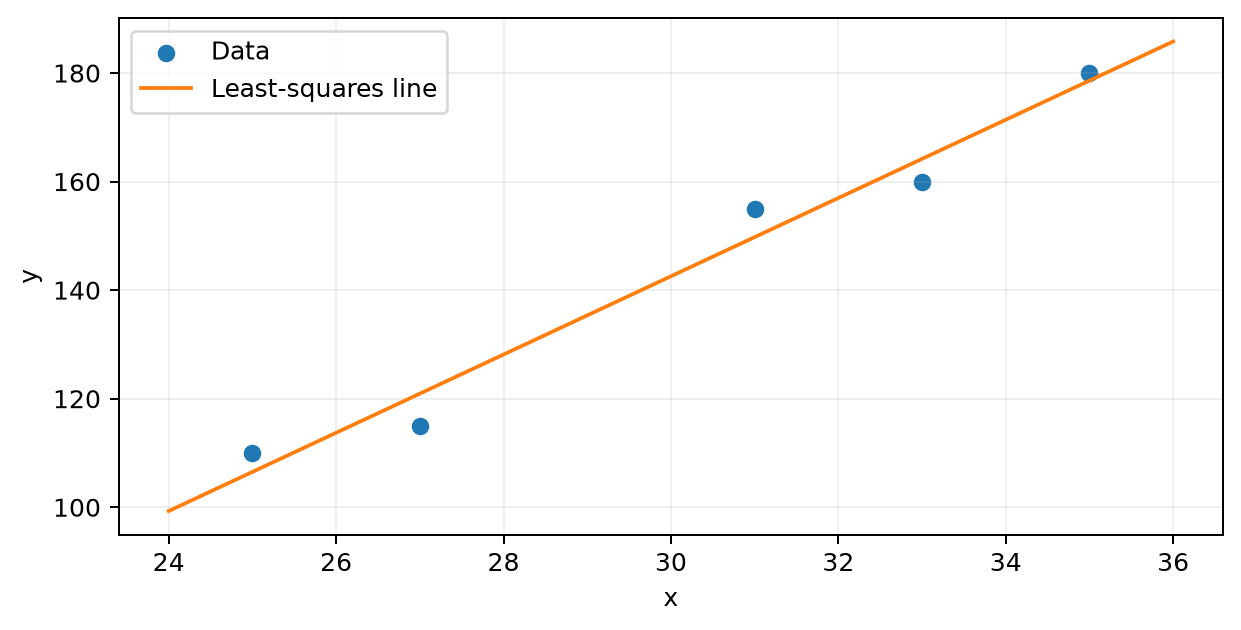
\includegraphics[width=\linewidth,height=64.77mm,keepaspectratio]{figures/linear_fit.png}\caption{The least squares line and all five supplied observations.}\end{figure}
The fit minimizes squared vertical deviations, not perpendicular distances to the line. The intercept is extrapolated far outside the observed x range 25 to 35, so it should not be interpreted as an observed response at x = 0. Residuals sum to zero and their x weighted sum is zero.

\clearpage
\section*{4 Experiment 1 3 population growth models}
Let t = year - 1790 in years, and u = t/100 in centuries. The constant rate model and variable rate model become linear least squares problems after taking natural logarithms. The scaling by 100 improves numerical conditioning without changing the fitted functions.

\[\log P=a+bt,\qquad P=P_0e^{rt},\quad P_0=e^a,\ r=b.\]
\[\log P=a+bt+ct^2,\qquad P=P_0e^{r_0t-r_1t^2/2},\quad r_0=b,\ r_1=-2c.\]
\[P_{\mathrm{constant}}(t)=6.5484411213\exp(0.01910297011t).\]
\[P_{\mathrm{variable}}(t)=3.8505777326\exp(0.03358489266t-0.000062964881t^2).\]
{\small\begin{tabular}{p{0.232\linewidth}p{0.232\linewidth}p{0.232\linewidth}p{0.232\linewidth}}\toprule
Model & Log RSS & Population RSS & Population RMSE\\\midrule
Constant rate & 1.7868471415 & 69236.899683 & 53.710993\\
Variable rate & 0.0482483254 & 1237.543300 & 7.180829\\
\bottomrule\end{tabular}}\par
\begin{figure}[H]\centering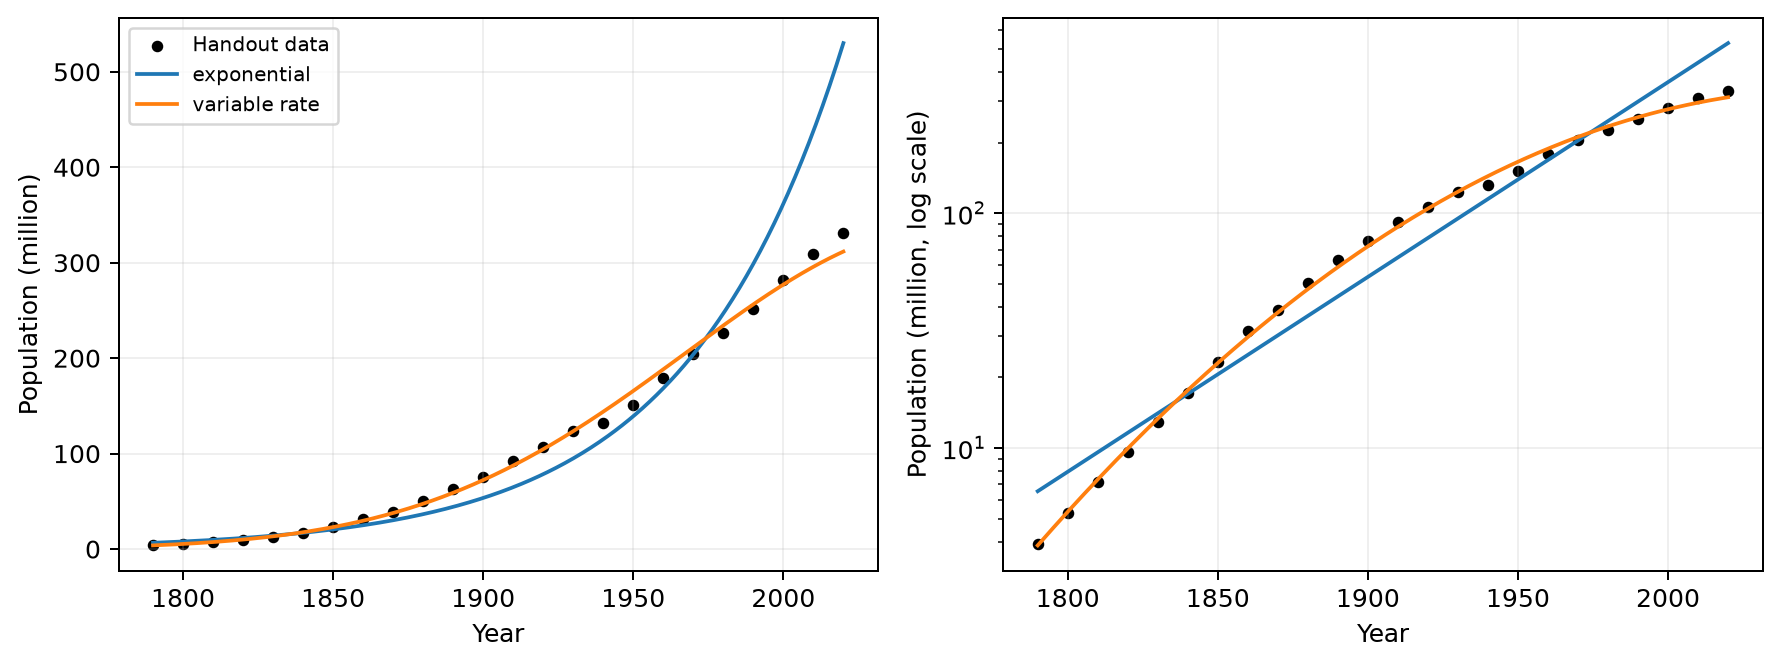
\includegraphics[width=\linewidth,height=57.15mm,keepaspectratio]{figures/population_models.png}\caption{Fits to the 24 supplied observations in linear and logarithmic population scales.}\end{figure}
Population is measured in millions. The primary objective is unweighted squared log error, not squared error in population units. The latter is reported as a separate diagnostic. The quadratic model reduces log RSS by 97.2998 percent. This extra flexibility does not establish accurate future extrapolation or a causal demographic law.

The variable rate model has instantaneous log growth r0 - r1 t. The fitted r1 is positive, so the modeled growth rate decreases over the observed period. Predictions and signed log residuals for every year are archived in population\_fits.csv.

\clearpage
\section*{5 Experiment 2 1 best linear approximation}
For f(x) = x squared on [0,1], minimize the integral of (x squared - c0 - c1 x) squared. Expanding and differentiating with respect to both coefficients gives:

\[E(c_0,c_1)=\frac15-\frac{2c_0}{3}-\frac{c_1}{2}+c_0^2+c_0c_1+\frac{c_1^2}{3}.\]
\[\begin{pmatrix}1&1/2\\1/2&1/3\end{pmatrix}\begin{pmatrix}c_0\\c_1\end{pmatrix}=\begin{pmatrix}1/3\\1/4\end{pmatrix}.\]
\[c_0=-\frac16,\quad c_1=1,\quad p(x)=x-\frac16,\quad \|x^2-p\|_2^2=\frac1{180}.\]
The two equations express zero inner products of the residual with 1 and x. The Gram determinant is 1/12 and the leading entry is positive, so the solution is the unique minimizer. The squared error equals 1/5 minus the inner product of f with its projection, namely 1/5 - 7/36 = 1/180.

\begin{figure}[H]\centering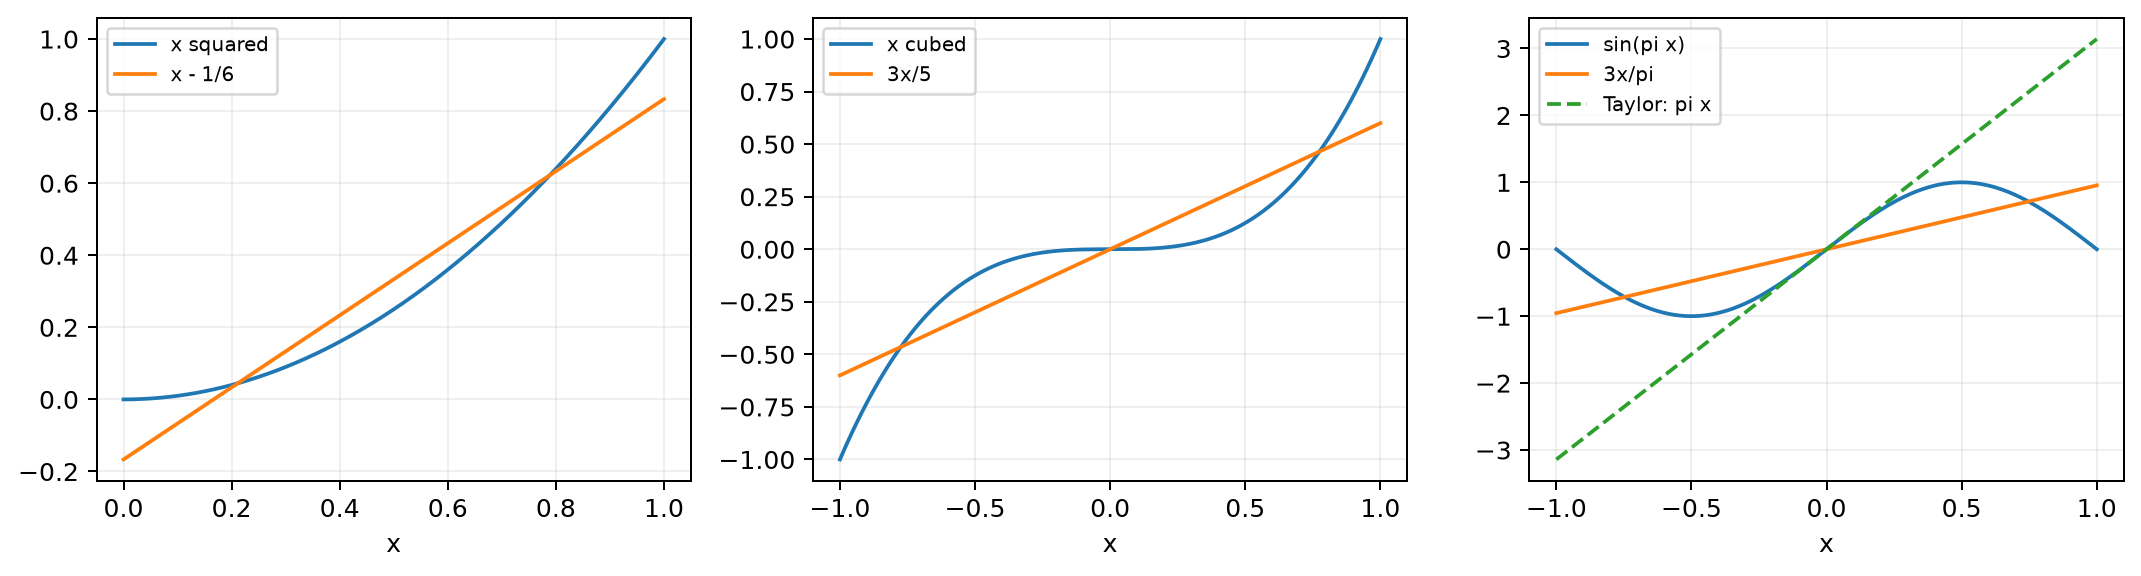
\includegraphics[width=\linewidth,height=59.69mm,keepaspectratio]{figures/continuous_approximations.png}\caption{Continuous projections for Experiments 2.1 to 2.3. The last panel also includes the Taylor polynomial.}\end{figure}
A best approximation may miss both endpoints. Here it takes values -1/6 and 5/6 at 0 and 1; those endpoint differences do not contradict its optimality for integrated error. The numerical quadrature check agrees with 1/180 to floating point precision.

\clearpage
\section*{6 Experiment 2 2 Legendre approximation}
On [-1,1], P0 = 1, P1 = x and P2 = (3x squared - 1)/2 form an orthogonal, but not normalized, basis. Their squared norms are 2, 2/3 and 2/5. Each coefficient is computed independently by dividing the corresponding inner product by the squared norm.

\[a_j=\frac{\langle x^3,P_j\rangle}{\langle P_j,P_j\rangle},\qquad (\langle x^3,P_0\rangle,\langle x^3,P_1\rangle,\langle x^3,P_2\rangle)=(0,2/5,0).\]
\[a_0=0,\qquad a_1=\frac{2/5}{2/3}=\frac35,\qquad a_2=0.\]
\[p_2=0P_0+\frac35P_1+0P_2=\frac35x.\]
The target x cubed is odd, while P0 and P2 are even. Their products are odd and integrate to zero over the symmetric interval, forcing both even coefficients to vanish. The degree at most two space permits a minimizer of degree one; the quadratic coefficient is not required to be nonzero.

\[\|x^3-p_2\|_2^2=\frac27-\frac{(2/5)^2}{2/3}=\frac8{175}.\]
The residual is orthogonal to all three basis polynomials, not merely to P1. An independent 160 point Gauss Legendre rule checks the Gram matrix, coefficient vector, residual inner products and the exact squared error. Orthogonal bases diagonalize the Gram system and avoid the coupling present in monomial coordinates.

\subsection*{Link with a higher Legendre mode}
\[P_3(x)=\frac12(5x^3-3x),\qquad x^3=\frac35P_1(x)+\frac25P_3(x).\]
Projection onto degrees zero through two drops the P3 component. Its squared norm is (2/5) squared times 2/7, which again gives 8/175. This provides a second analytic check.

\clearpage
\section*{7 Experiment 2 3 quadratic fit to sine}
With the monomial basis 1, x, x squared on [-1,1], parity makes odd moments zero. Integration by parts gives the only nonzero right hand side entry, the inner product of x and sin(pi x), equal to 2/pi.

\[\begin{pmatrix}2&0&2/3\\0&2/3&0\\2/3&0&2/5\end{pmatrix}\begin{pmatrix}c_0\\c_1\\c_2\end{pmatrix}=\begin{pmatrix}0\\2/\pi\\0\end{pmatrix}.\]
\[c_0=c_2=0,\quad c_1=\frac3\pi,\quad p_2(x)=\frac3\pi x.\]
The even coefficient block has determinant 16/45, so its homogeneous equations force both even coefficients to zero. This is also required because the target is odd and the projection onto a symmetric polynomial space preserves parity.

\[\|\sin(\pi x)-p_2\|_2^2=1-\frac6{\pi^2}=0.3920728981.\]
\[T_2(x)=\pi x,\qquad \|\sin(\pi x)-T_2\|_2^2=\frac{2\pi^2}{3}-3=3.579736267.\]
The Taylor polynomial of degree two has no constant or quadratic term, but its slope pi differs from the projection slope 3/pi. Taylor matches derivatives locally at zero. The projection minimizes the integrated squared error over the entire interval and therefore has a much smaller total squared error. A Taylor term of degree three would be a different polynomial outside the assigned degree at most two space.

The sine squared integral equals 1. For any scalar slope a, the squared error is 1 - 4a/pi + 2a squared/3; substitution of a = 3/pi or a = pi gives the two exact errors above. This verifies the comparison without relying on plotting.

\clearpage
\section*{8 Experiment 3 1 airfoil approximation}
The 129 coordinates are ordered from the trailing edge along the lower branch to the leading edge, then back along the upper branch. Split at the minimum x, sharing the leading edge; each branch contains 65 points. The small positive ordinates near the trailing edge belong to the lower branch and are not reassigned by sign.

\[g_1(x)=\sqrt{x}-x,\qquad g_i(x)=x^{i-1}(1-x),\quad i=2,3,4.\]
\[B_{ji}=g_i(x_j),\qquad \widehat{\alpha}=\arg\min_\alpha\|B\alpha-y\|_2^2.\]
{\small\begin{tabular}{p{0.3153333333333333\linewidth}p{0.3153333333333333\linewidth}p{0.3153333333333333\linewidth}}\toprule
Coefficient & Upper branch & Lower branch\\\midrule
1 & 0.13068978718 & -0.12890279467\\
2 & 0.09878194827 & -0.10645607131\\
3 & 0.12688517233 & -0.18696393328\\
4 & -0.09259206959 & 0.42287649175\\
\bottomrule\end{tabular}}\par
{\small\begin{tabular}{p{0.182\linewidth}p{0.182\linewidth}p{0.182\linewidth}p{0.182\linewidth}p{0.182\linewidth}}\toprule
Branch & Points & RSS & RMSE & Max residual\\\midrule
upper & 65 & 1.357448018e-06 & 1.445123374e-04 & 3.129364589e-04\\
lower & 65 & 1.485217220e-05 & 4.780114610e-04 & 1.101830302e-03\\
\bottomrule\end{tabular}}\par
\begin{figure}[H]\centering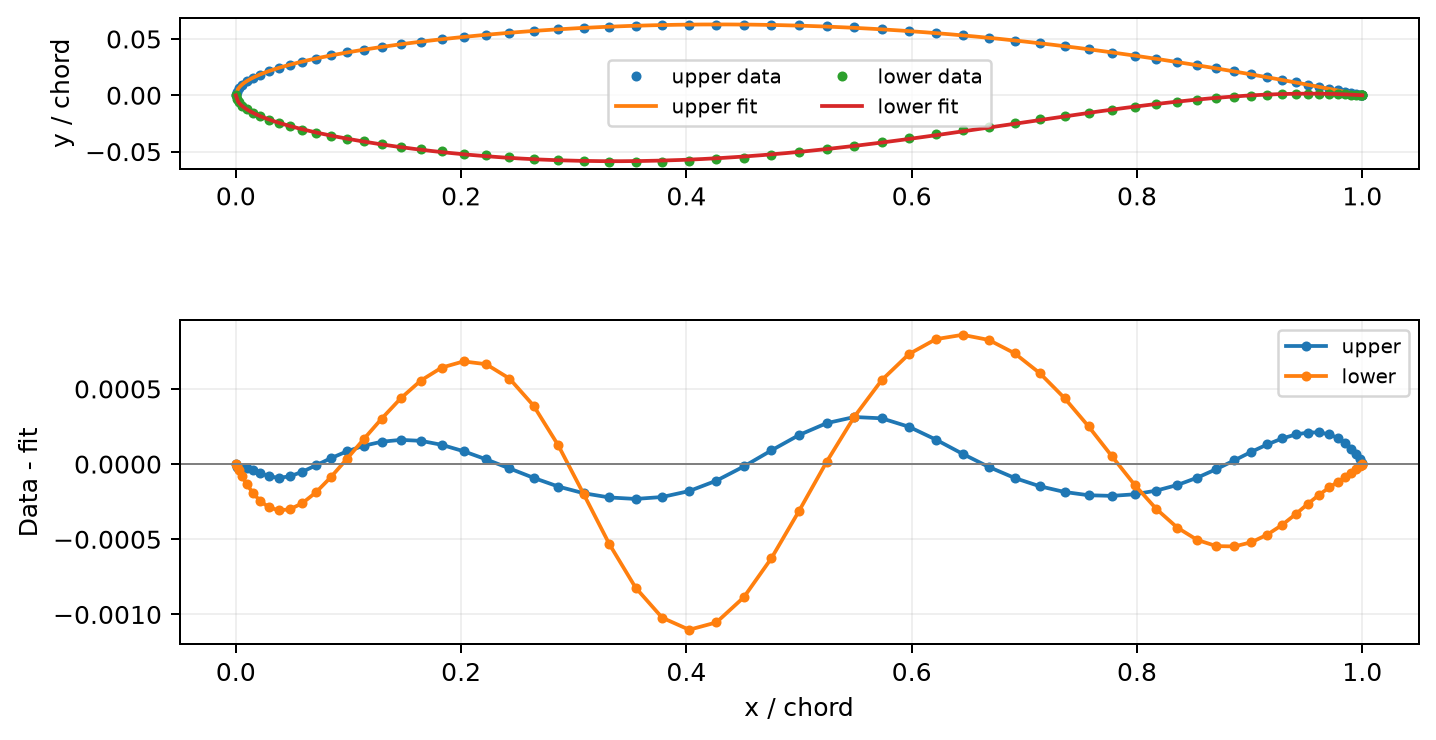
\includegraphics[width=\linewidth,height=66.03999999999999mm,keepaspectratio]{figures/airfoil_fit.png}\caption{Upper and lower fits with equal axis scaling in the geometry panel, and signed coordinate residuals below.}\end{figure}
All four basis functions vanish at both endpoints, enforcing leading and trailing edge closure. The lower branch has the larger residual. Endpoint rows are zero and do not identify coefficients, but the remaining rows have rank four. The residuals are ordinate errors in chord units, not orthogonal distances to a geometric curve. The experiment assesses geometric fit, not aerodynamic lift or drag.

\clearpage
\section*{9 Validation and reproducibility}
All 38 of 38 numerical checks pass. The checks compare every coordinate and population row with the supplied PDF, verify exact rational solutions, use independent LAPACK QR/SVD references, check projection orthogonality, and validate the CSV results.

{\small\begin{tabular}{p{0.232\linewidth}p{0.232\linewidth}p{0.232\linewidth}p{0.232\linewidth}}\toprule
Case & Condition A & Condition A T A & QR vs NumPy\\\midrule
Literal system & 3.0088 & 9.053 & 1.78e-15\\
Line fit & 249.84 & 62422 & 1.71e-13\\
Constant log model & 3.783 & 14.311 & 1.11e-15\\
Variable log model & 18.621 & 346.74 & 2.00e-15\\
Upper airfoil & 80.218 & 6435 & 1.39e-16\\
Lower airfoil & 80.218 & 6435 & 8.33e-17\\
\bottomrule\end{tabular}}\par
For the variable rate model, changing time units from years to centuries reduces the design condition number from 67564.163 to 18.621031. The coefficient transformation back to years is checked independently. Agreement on these examples does not remove the general instability of normal equations for ill conditioned designs.

From the package root, run python reproduce.py to regenerate numerical results, verification, figures, report content, the LaTeX PDF and the editable Word document. See README.md for the individual commands and directory layout. The final PDF is compiled from LaTeX before Word generation; the Word document uses native editable Office equations.

{\small\begin{tabular}{p{0.482\linewidth}p{0.482\linewidth}}\toprule
Runtime item & Recorded value\\\midrule
python & 3.13.7 (main, Aug 14 2025, 11:12:11) [Clang 17.0.0 (clang-1700.3.19.1)]\\
numpy & 2.5.3\\
scipy & 1.18.1\\
matplotlib & 3.11.2\\
\bottomrule\end{tabular}}\par
Source: the supplied seven page course PDF, preserved byte for byte. The alternative equation in Experiment 1.1 is reported explicitly as a possible correction, not as the authoritative statement. All 24 population values and all 129 airfoil coordinates are supplied observations; fitting them is not a new measurement of population or airfoil performance.

\end{document}